\documentclass[orientation=landscape]{tikzposter}
\usepackage{amsmath}
\usepackage{amsthm}
\usepackage{amssymb}

\geometry{paperwidth=48in,paperheight=36in}
\makeatletter
\setlength{\TP@visibletextwidth}{\textwidth-2\TP@innermargin}
\setlength{\TP@visibletextheight}{\textheight-2\TP@innermargin}
\makeatother

%%%%%%%%%%%%%%%%%%%%%%%%%%%%%
%%%			Title and Authors			%%%
%%%%%%%%%%%%%%%%%%%%%%%%%%%%%
\title{\parbox{\linewidth}{\centering On Modifications to Laguerre's Method and the Polynomial Eigenvalue Problem}}
\author{Thomas R. Cameron* \& Nikolas I. Steckley**}
\institute{Davidson College* \& DiscoverOrg LLC.**}
\usetheme{Rays}
\usebackgroundstyle{Default}
\usetitlestyle{Default}
%%%%%%%%%%%%%%%%%%%%%%%%%%%%%
%%%			Main Document				%%%
%%%%%%%%%%%%%%%%%%%%%%%%%%%%%
\begin{document}
	\maketitle
	%%%	Abstract	%%%
	\block{Abstract}{Laguerre's method has long been recognized for its strong virtues when computing the roots of a polynomial. Over the years, many modifications to Laguerre's method have been suggested in an attempt to improve its convergence rate and to avoid multiple convergence to a simple root. Now, we present a modification to Laguerre's method for the simultaneous convergence of all roots of a polynomial. Multiple numerical experiments verify both the accuracy and efficiency of this algorithm, and we provide comparisons to other root finding methods, such as POLZEROS and AMVW. Furthermore, we are able to apply this method to the polynomial eigenvalue problem, where it is effective for large degree problems, and the Tridiagonal problem.}
	%%%	Column 1	%%%
	\begin{columns}
		\column{0.333}
		%%%	Introduction	%%%
		\block{Introduction}{
			Let $p(\lambda)$ be a polynomial of degree $m$. Denote by $(z_{1},\ldots,z_{m})$ current approximations to the roots, $r_{1},\ldots,r_{m}$ of $p(\lambda)$. Then, for $j\in\{1,\dots,m\}$ define
			\[
			f_{j}(\lambda)=\frac{p(\lambda)}{\prod\limits_{\substack{i=1\\i\neq j}}^{m}(\lambda-z_{i})},
			\]
			and note that $f_{j}(\lambda)$ has the same roots as $p(\lambda)$. Further define
			\begin{equation}
			\begin{split}
			G_{j}(\lambda)&=\frac{f_{j}^{'}(\lambda)}{f_{j}(\lambda)}=\frac{p^{'}(\lambda)}{p(\lambda)}-\sum_{\substack{i=1\\i\neq j}}^{m}\frac{1}{\lambda-z_{i}}, \\
			H_{j}(\lambda)&=-\left(\frac{f_{j}^{'}(\lambda)}{f_{j}(\lambda)}\right)^{'}=-\left(\frac{p^{'}(\lambda)}{p(\lambda)}\right)^{'}-\sum_{\substack{i=1\\i\neq j}}^{m}\frac{1}{(\lambda-z_{i})^{2}}.
			\end{split}
			\end{equation}
			Then the jth root approximation is updated via the expression
			\begin{equation}\label{eq:lag2}
			\hat{z}_{j}=z_{j}-L_{m}(z_{j}),
			\end{equation}
			where the modified Laguerre updated is defined by
			\begin{equation}
			L_{m}(z_{j})=\frac{m}{G_{j}(z_{j})\pm\sqrt{(m-1)(mH_{j}(z_{j})-G_{j}^{2}(z_{j}))}},
			\end{equation}
			and the sign is chosen to maximize the magnitude of the denominator. \\
			The removal of previously computed roots is a well known modification of Laguerre's method and has been employed in~\cite{Lancaster1966,Parlett1964}. Here, we create poles at $z_{1},\ldots,z_{j-1},z_{j+1},\ldots,z_{m}$ in order to direct the Laguerre iteration away from other root approximations. A similar idea was used by Aberth to modify Newton's method~\cite{Aberth1973}. This makes for an algorithm that simultaneously approximates all roots of a polynomial. 
		}
		%%%	Algorithm Outline	%%%
		\block{Algorithm Outline}{
			For $j=1,\ldots,m$, the $jth$ root approximation is updated via (2), provided that it is not already close enough to the root $r_{j}$. The iteration can be implemented in either a Jacobi style (can be parallelized) or in a Gauss-Seidel style (experiences slightly faster convergence). Our current algorithm (DSLM) uses a Gauss-Seidel iteration style and has the following attributes.\\
			\textbf{Order of Convergence.}	Locally, if the root is simple, convergence is quartic; otherwise it is linear. \\
			\textbf{Cost Complexity.}	The computation of both expressions in (1) requires the evaluation of $p(\lambda)$, $p^{'}(\lambda)$, and $p^{''}(\lambda)$, along with the evaluation of two sums; this can be done in $O(m)$ time. The convergence of all roots requires $O(m)$ iterations, it follows that DSLM can compute all root approximations in $O(m^{2})$ time. 
		}
		%%%	Column 2	%%%	
		\column{0.333}
		%%%	Initial Estimates		%%%
		\block{Initial Estimates}{
			Let $p(\lambda)=\sum_{i=0}^{m}a_{i}\lambda^{i}$, where $a_{0}a_{m}\neq 0$. The \emph{Newton polygon} associated with this polynomial is the upper convex hull of the discrete set $\{(i,\log|a_{i}|\colon~i=0,1,\ldots,m\}$. Let $0=k_{0}<k_{1}<\cdots<k_{q}=m$ denote the abscissas of the vertices of the Newton polygon, and define the radii
			\[
			\mu_{i}=\left|\frac{a_{k_{i-1}}}{a_{k_{i}}}\right|^{\frac{1}{k_{i}-k_{i-1}}},~(i=1,\ldots,q).
			\]
			Then, $(k_{i}-k_{i-1})$ evenly distributed points are placed on circles centered at $0$ with radius $\mu_{i}$. These points constitute our initial estimates to the roots of $p(\lambda)$. Furthermore, these points are guaranteed to lie within the Pellet bounds for the polynomial $p(\lambda)$, and can be computed in $O(m\log m)$ time~\cite{Bini1996}.
		}
		%%%	Stopping Criteria	%%%
		\block{Stopping Criteria}{
			It follows from~\cite{Tisseur2000}[Lemma 3] that the backward error in the root approximation $z_{j}$ is bounded above by
			\[
				b(z_{j})=\frac{|p(z_{j})|}{\sum\limits_{i=0}^{m}|a_{i}||z_{j}|^{i}}.
			\]
			If $b(z_{j})<\epsilon$, where $\epsilon$ denotes double precision unit roundoff, then we say that the approximation $z_{j}$ has converged. This constitutes our first stopping criterion. Otherwise, we compute the modified Laguerre update (3). If $|L_{m}(z_{j})|<\epsilon|z_{j}|$, then no relatively significant contribution will be made by $L_{m}(z_{j})$ and we say that the approximation $z_{j}$ has converges. This constitutes our second stopping criterion. Otherwise, we update $z_{j}$ via (2). 
		}
		%%%	Comparison to Aberth and Laguerre	%%%
		\block{Comparison to Aberth and Laguerre}{
			\centering
			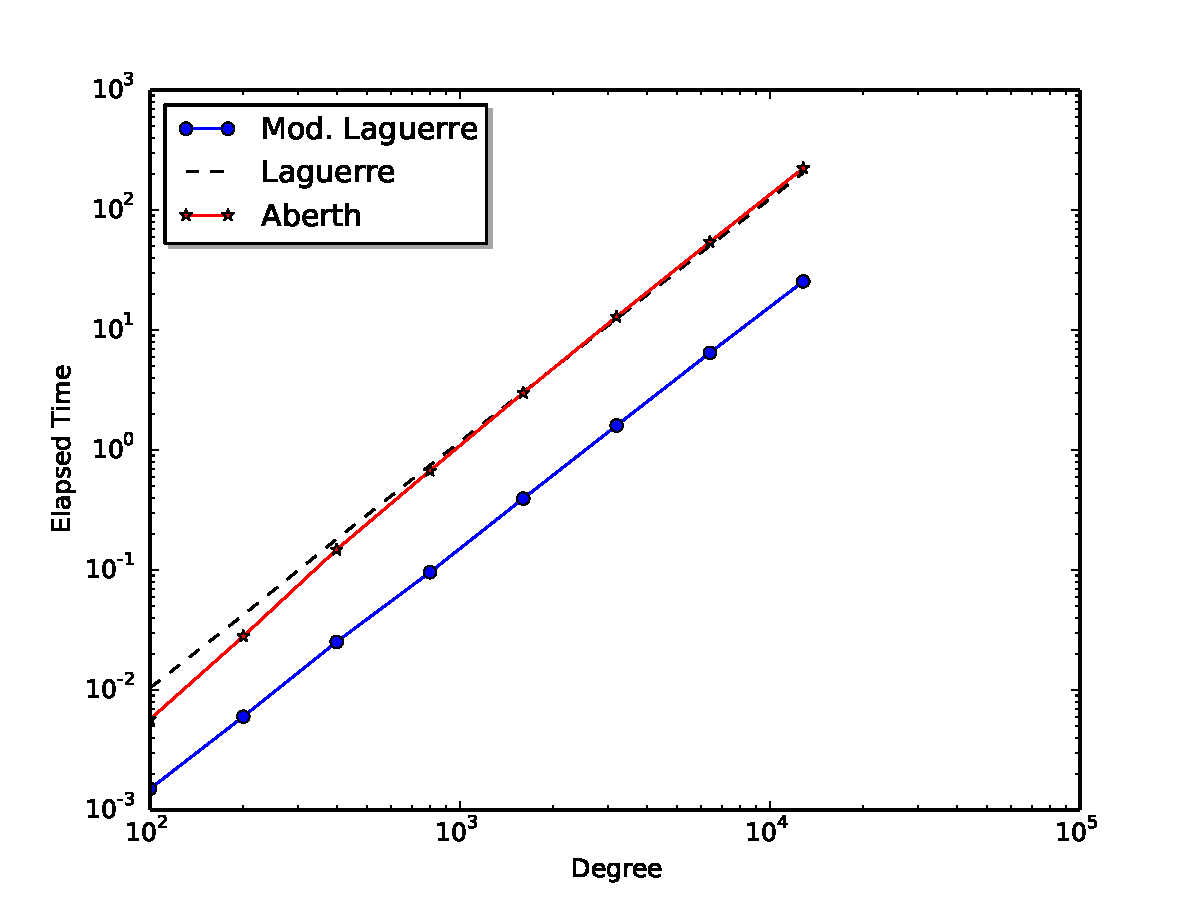
\includegraphics[scale=1.0]{../develop/tests/diagrams/testMethods.pdf}
		}
		%%%	Column 3	%%%
		\column{0.333}
		%%%	Comparison to POLZEROS and AMVW	%%%
		\block{Comparison to POLZEROS and AMVW}{
			\centering
			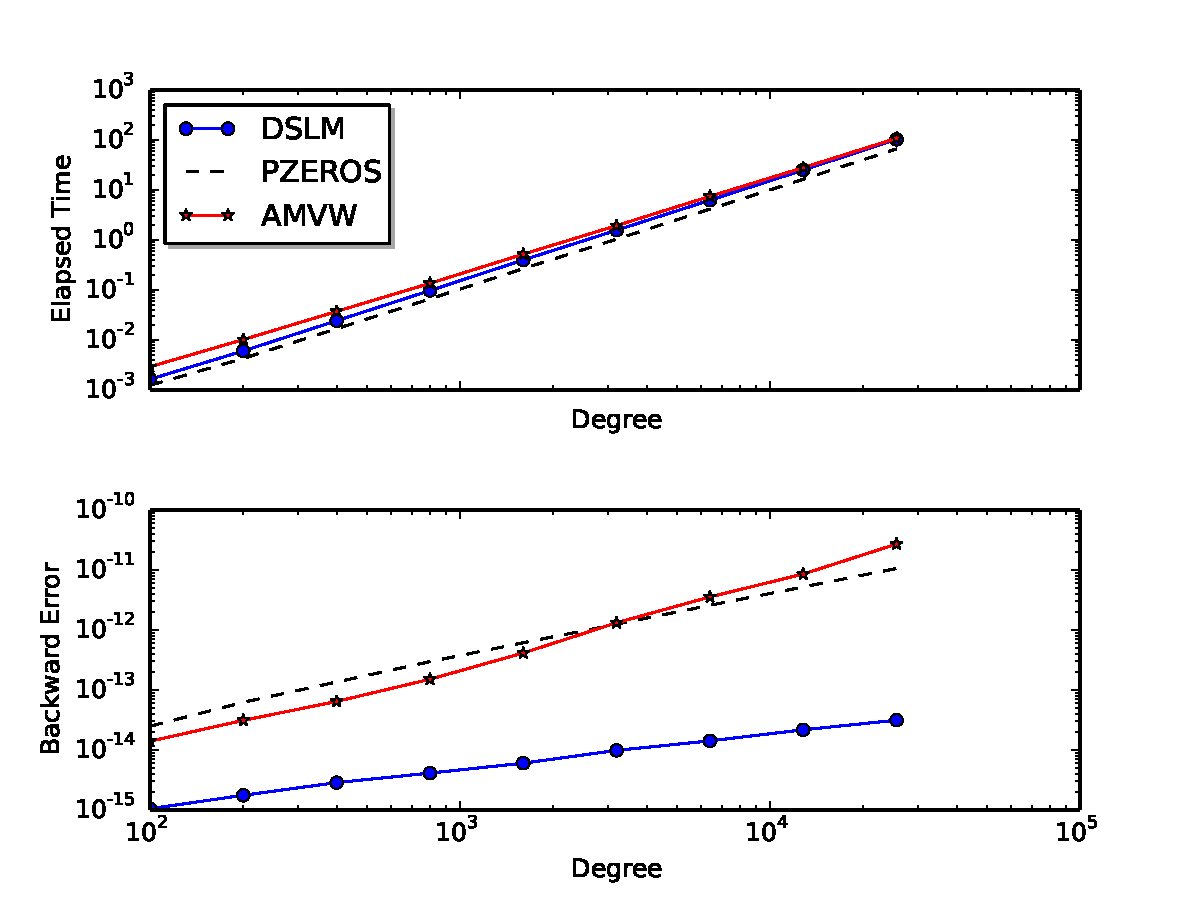
\includegraphics[scale=1.0]{../develop/tests/diagrams/testComparison1.pdf}\\
			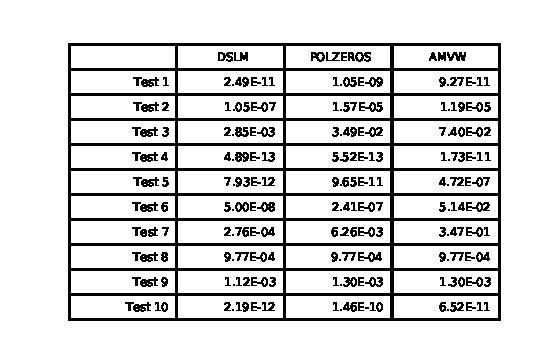
\includegraphics[scale=2.0]{../develop/tests/diagrams/testComparison2.pdf}
		}
		\block{Conclusion}{
			Future research includes applying this modified Laguerre method to the polynomial eigenvalue problem. 
			%%%	References	%%%
			\bibliographystyle{siam}
			\bibliography{Bibliography}		
		}
	\end{columns}
\end{document}